\documentclass{article}
\usepackage[utf8]{inputenc}
\usepackage{graphicx}
\usepackage{fancyhdr}
\usepackage{geometry}
\usepackage{amsmath}
\usepackage{amssymb}


\geometry{left = 2.5cm, right=2.5cm, bottom=2.5cm, top=2.5cm}

\title{Building a Neural Network to Recognise Handwriting}
\author{Nick van der Merwe - s5151332 - nick.vandermerwe\@griffithuni.edu.au}

\pagestyle{fancy}
\renewcommand{\headrulewidth}{1pt}
\fancyhf{}
\rhead{2802ICT - Assignment 2}
\chead{Griffith University}
\lhead{Nick van der Merwe - s5151332}
\rfoot{Page \thepage}

\begin{document}
\maketitle

%==============================================================================
\section{Introduction}
In this report a model for predicting hand writing digits was built from the
ground up excluding its prepocessing. The dataset used was MNIST, and it
achieved a peak accuracy of 94.45\%. The approach was to build a small neural
network manually and calculate its values by hand, then scaling this up to the
MNIST set all in Python with NumPy.

\section{Calculating a neural network by hand}
We were tasked to do a neural network's calculations by hand through stochastic
gradient descent with backpropagation. Note that in the next section there is a
summary table of the weights that were produced (page 18).

\begin{figure}[ht]
    \centering
    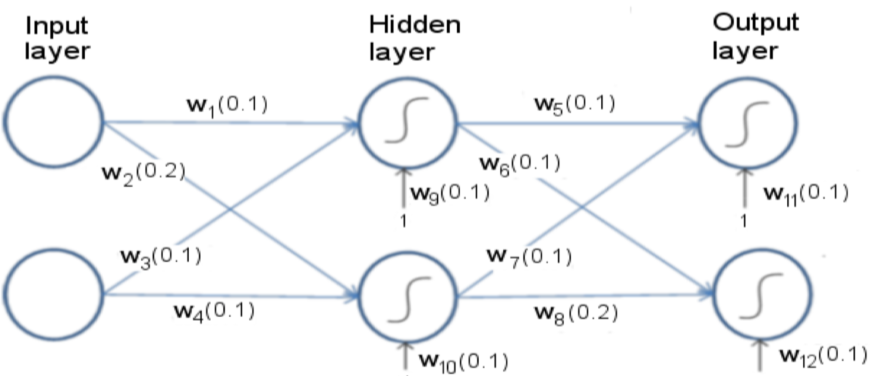
\includegraphics[scale=0.5]{neurelNetwork.png}
    \caption{
        Neural Network to update weights for. We'll nickname the layers i1, i2
        (input), h1, h2 (hidden), o1, o2 (output). Where 1 signs the top and 2
        the bottom
    }
    \label{NN}
\end{figure}

\begin{equation*}
  \begin{array}{l}
    Batch \; size = 2 \qquad Learning \; Rate = 0.1 \\
    Samples: \; X_{1} = (0.1, \; 0.1); \quad X_{2} = (0.1, \; 0.2); \\
    \qquad \qquad \; \; \; \; Y_{1} = (1, \; 0); \qquad \; \; \;  Y_{2} = (0, \; 1);
  \end{array}
\end{equation*}

Now that all our variables have been finished we can move onto the first
forwards pass

\newpage
\subsection{Forwards Pass 1}

\subsubsection{$out_{h1}$}
Since this is the first out that will be calculated, a few formulas will be
defined here. Then from this point onwards the values will simply be plugged
into the equations.

\begin{align*}
    net_{h1} & = w_{1} \times i_1 + w_{3} \times i_{2} + b_{1} \times w_{11} \\
           & = 0.1 \times 0.1 + 0.1 \times 0.1 + 1 \times 0.1 \\
           & = 0.12
\end{align*}

Now to find $out_{h1}$ we use the sigmoid function

\begin{align*}
    out_{h1} = \sigma(net_{h1}) & = \frac{1}{1 + e^{-net_{h1}}} \\
 &= 0.5299640517645717
\end{align*}

\subsubsection{$out_{h2}$}
\begin{align*}
    net_{h2} & = w_{2} \times i_1 + w_{4} \times i_{2} + b_{2} \times w_{10} \\
    & = 0.2 \times 0.1 + 0.1 \times 0.1 + 0.1 \times 1 \\
    & = 0.13
\end{align*}

\begin{align*}
    out_{h2} = \sigma(net_{h2}) & = \frac{1}{1 + e^{-net_{h2}}} \\
 &= 0.5324543063873187
\end{align*}

\subsubsection{$out_{o1}$}

\begin{align*}
    net_{o1} & = w_{5} \times out_{h1} + w_{7} \times out_{h2} + b_{2} \times w_{11} \\
    & = 0.1 \times 0.5299640517645717 + 0.1 \times  0.5324543063873187 + 0.1 \times 1 \\
    & = 0.20624183581518907
\end{align*}

\begin{align*}
    out_{o1} = \sigma(net_{o1}) & = \frac{1}{1 + e^{-net_{o1}}} \\
    & = 0.5513784696896066
\end{align*}

\subsubsection{$out_{o2}$}
\begin{align*}
    net_{o2} & = w_{6} \times out_{h1} + w_{8} \times out_{h2} + b_{2} \times w_{12} \\
    & = 0.1 \times 0.5299640517645717 + 0.2 \times  0.5324543063873187 + 0.1 \times 1 \\
    & =  0.25948726645392095
\end{align*}

\begin{align*}
    out_{o2} = \sigma(net_{o2}) & = \frac{1}{1 + e^{-net_{o2}}} \\
    & = 0.5645102463659317
\end{align*}

%%%%%%%%%%%%%%%%%%%%%%%%%%%%%%%%%%%%%%%%%%%%%%%%%%%%%%%%%%%%%%%%%%%%%%%%%%%%%%%
\subsection{Error}
\begin{align*}
    E_{total} & = \sum \frac{1}{2} (target-output)^2 \\
    E_{o1} & = \frac{1}{2}(1-0.5513784696896066)^2 = 0.10063063872901962 \\
    E_{o2} & = \frac{1}{2}(1-0.5645102463659317)^2 = 0.15933590912606246 \\
    E_{total} & = E_{o1} + E_{o2} = 0.2527076596804409
\end{align*}

%%%%%%%%%%%%%%%%%%%%%%%%%%%%%%%%%%%%%%%%%%%%%%%%%%%%%%%%%%%%%%%%%%%%%%%%%%%%%%%
\subsection{Backwards Pass 1 - Output Layer}
Since it can be easy to make mistakes, there won't be any shortcuts - e.g. start
declaring each part individually. Instead, we will do this in detail. The last
section for these will contain a summary of the values though.
\subsubsection{$\frac{\partial E_{total}}{\partial w_5}$}

\begin{align*}
    \frac{\partial E_{total}}{\partial w_5} & =
    \frac{\partial E_{total}}{\partial out_{o1}} \times
    \frac{\partial out_{o1}}{\partial net_{o1}} \times
    \frac{\partial net_{o1}}{\partial w_5} 
\end{align*}
\begin{align*}
    \frac{\partial E_{total}}{\partial out_{o1}} =
    & = 2 \times \frac{1}{2}(target_{o1} - out_{o1})^{2 - 1} \times -1 + 0 \\
    & = -(1- 0.5513784696896066)= -0.4486215303103934
\end{align*}
\begin{align*}
    \frac{\partial out_{o1}}{\partial net_{o1}} & =
    out_{o1}(1 - out_{o1}) = 0.5513784696896066(1- 0.5513784696896066) \\
    & =0.2473602528523542
\end{align*}
\begin{align*}
    \frac{\partial net_{o1}}{\partial w_5} & = 
    out_{h1} = 0.5299640517645717
\end{align*}
\begin{align*}
    \frac{\partial E_{total}}{\partial w_5} & =
    \frac{\partial E_{total}}{\partial out_{o1}} \times
    \frac{\partial out_{o1}}{\partial net_{o1}} \times
    \frac{\partial net_{o1}}{\partial w_5} \\
    & = -0.4486215303103934 \times 0.2473602528523542 \times 0.5299640517645717 \\
    & = -0.05881071242497923
\end{align*}

\subsubsection{$\frac{\partial E_{total}}{\partial w_7}$}
For this we just have to define that $
    \frac{\partial net_{o1}}{\partial w_5} = out_{h2} = 0.5324543063873187
$ and replace it in the previous formula
\begin{align*}
    \frac{\partial E_{total}}{\partial w_7} & =
    \frac{\partial E_{total}}{\partial out_{o1}} \times
    \frac{\partial out_{o1}}{\partial net_{o1}} \times
    \frac{\partial net_{o1}}{\partial w_7} \\
    & = -0.4486215303103934 \times 0.2473602528523542 \times 0.5324543063873187
    \\
    & =-0.05908705880733
\end{align*}

\subsubsection{$\frac{\partial E_{total}}{\partial w_{11}}$}
*side note: The bias weights would have been found first, but since they are not
in the exemplar... they are here now.
Granted that this is a bias weight, its value for$
    \frac{\partial net_{o1}}{\partial w_{11}} 
$ is just $1$, we are going to take the previous value and divide it by its 
$\frac{\partial net_{o1}}{\partial w_7} $ value. This will be done for all the
bias weights.
\begin{align*}
    \frac{\partial E_{total}}{\partial w_{11}} 
    & = \frac{-0.05908705880733}{0.5324543063873187} \\
    & = -0.1109711351725809
\end{align*}


\subsubsection{$\frac{\partial E_{total}}{\partial w_6}$}

\begin{align*}
    \frac{\partial E_{total}}{\partial w_6} & =
    \frac{\partial E_{total}}{\partial out_{o2}} \times
    \frac{\partial out_{o2}}{\partial net_{o2}} \times
    \frac{\partial net_{o2}}{\partial w_6} 
\end{align*}
\begin{align*}
    \frac{\partial E_{total}}{\partial out_{o2}}
    & = 2 \times \frac{1}{2}(target_{o2} - out_{o2})^{2 - 1} \times -1 + 0 \\
    & = -(0- 0.5645102463659317) \\ & = 0.56451024636593174
\end{align*}
\begin{align*}
    \frac{\partial out_{o2}}{\partial net_{o2}} 
    & = out_{o1}(1 - out_{o1}) = 0.5645102463659317(1- 0.5645102463659317) \\
    & =0.2458384281138062
\end{align*}
\begin{align*}
    \frac{\partial net_{o2}}{\partial w_6} 
    & = out_{h1} =  0.52996405176457177
\end{align*}
\begin{align*}
    \frac{\partial E_{total}}{\partial w_6} & =
    \frac{\partial E_{total}}{\partial out_{o2}} \times
    \frac{\partial out_{o2}}{\partial net_{o2}} \times
    \frac{\partial net_{o2}}{\partial w_6} \\
    & = 0.5645102463659317 \times 0.245838428113806 \times 0.5299640517645717 \\
    & = 0.073547516323
\end{align*}

\subsubsection{$\frac{\partial E_{total}}{\partial w_8}$}
For this we just have to define that $
    \frac{\partial net_{o2}}{\partial w_8} = out_{h2} = 0.5324543063873187
$ and replace it in the previous formula
\begin{align*}
    \frac{\partial E_{total}}{\partial w_8} & =
    \frac{\partial E_{total}}{\partial out_{o2}} \times
    \frac{\partial out_{o2}}{\partial net_{o2}} \times
    \frac{\partial net_{o2}}{\partial w_8} \\
    & = 0.5645102463659317 \times 0.2458384281138062 \times 0.5324543063873187
    \\
    & =0.07389310965563
\end{align*}

\subsubsection{$\frac{\partial E_{total}}{\partial w_{12}}$}
This is a bias weight, so we will reverse the previous operation.
\begin{align*}
    \frac{\partial E_{total}}{\partial w_12} & = 
    \frac{\partial E_{total}}{\partial w_8} /
    \frac{\partial net_{o2}}{\partial w_8} \\
    & = \frac{0.07389310965563}{0.5324543063873187} \\
    & = 0.138778311620750729
\end{align*}


\subsubsection{Summary of Values}
\begin{align*}
    \frac{\partial E_{total}}{\partial w_5} &= -0.05881071242497923 \\
    \frac{\partial E_{total}}{\partial w_6} &= 0.0735475163237 \\
    \frac{\partial E_{total}}{\partial w_{11}} &= -0.1109711351725809 \\
    \frac{\partial E_{total}}{\partial w_7} &= -0.05908705880733 \\
    \frac{\partial E_{total}}{\partial w_8} &= 0.073893109655633 \\
    \frac{\partial E_{total}}{\partial w_12} & = 0.138778311620750729 \\
\end{align*}
%%%%%%%%%%%%%%%%%%%%%%%%%%%%%%%%%%%%%%%%%%%%%%%%%%%%%%%%%%%%%%%%%%%%%%%%%%%%%%%
\subsection{Backwards Pass 1 - Hidden Layer}
\subsubsection{$\frac{\partial E_{total}}{\partial w_1}$}
\begin{align*} \frac{\partial E_{total}}{\partial w_1} & =
    \frac{\partial E_{total}}{\partial out_{h1}} \times
    \frac{\partial out_{h1}}{\partial net_{h1}} \times
    \frac{\partial net_{h1}}{\partial w_1}
\end{align*}
\\
However, since the hidden layer affects this layer our formula for the $
    \frac{\partial E_{total}}{\partial_{h1}}
$ is different. Now it's:
\begin{align*}
    \frac{\partial E_{total}}{\partial out_{h1}} & = 
    \frac{\partial E_{o1}}{\partial out_{h1}} +
    \frac{\partial E_{o2}}{\partial out_{h1}}
\end{align*}
And these are also defined as:
\begin{align*}
    \frac{\partial E_{o1}}{\partial out_{h1}} & =
    (\frac{\partial E_{o1}}{\partial net_{o1}}) \times
    \frac{\partial net_{o1}}{\partial out_{h1}}
    = (\frac{\partial E_{o1}}{\partial out_{o1}} \times
        \frac{\partial out_{o1}}{\partial net_{o1}} ) \times w_5 \\
    & = -0.4486215303103934 \times 0.2473602528523542 \times 0.1 \\
    & = -0.0110971135172588
\end{align*}
\begin{align*}
    \frac{\partial E_{o2}}{\partial out_{h1}} & =
    (\frac{\partial E_{o2}}{\partial net_{o2}}) \times
    \frac{\partial net_{o2}}{\partial out_{h1}} 
    = (\frac{\partial E_{o2}}{\partial out_{o2}} \times
        \frac{\partial out_{o2}}{\partial net_{o2}} ) \times w_6 \\
    &= 0.5645102464 \times 0.2458388281 \times 0.1 \\
    & = 0.013877854573
\end{align*}

Which gives us:
\begin{align*}
    \frac{\partial E_{total}}{\partial out_{h1}} & = 
    \frac{\partial E_{o1}}{\partial out_{h1}} +
    \frac{\partial E_{o2}}{\partial out_{h1}} \\
    & =  -0.0110971135172588 + 0.013877854573 \\
    & = 0.0027807410557412
\end{align*}

Now we can move back into defining the rest of the formula
\begin{align*}
    \frac{\partial out_{h1}}{\partial net_{h1}} & =
    out_{h1}(1 - out_{h1}) = 0.5299640517645717(1-0.5299640517645717) \\
    & = 0.2491021556018500
\end{align*}

\begin{align*}
    \frac{\partial net_{h1}}{\partial w_1} & = 
    out_{i1} = in_{1} = 0.1
\end{align*}

\begin{align*}
    \frac{\partial E_{total}}{\partial w_1} & =
    \frac{\partial E_{total}}{\partial out_{h1}} \times
    \frac{\partial out_{h1}}{\partial net_{h1}} \times
    \frac{\partial net_{h1}}{\partial w_1} \\
    & = 0.0027807410557412 \times 0.2491021556018500 \times 0.1 \\
    & = 0.0000692688591155
\end{align*}

\subsubsection{$\frac{\partial E_{total}}{\partial w_3}$}
We can do a similar shortcut to the output layer since this shares a lot of
variables with the previous subsubsection.
\begin{align*} 
    \frac{\partial E_{total}}{\partial w_3} & =
    \frac{\partial E_{total}}{\partial out_{h1}} \times
    \frac{\partial out_{h1}}{\partial net_{h1}} \times
    \frac{\partial net_{h1}}{\partial w_3} \\
\end{align*}
The only different variable is the third multiple, and this is:
\begin{align*}
    \frac{\partial net_{h1}}{\partial w_3} & = 
    out_{i2} = in_{2} = 0.1 =
    \frac{\partial net_{h1}}{\partial w_1} \\
\end{align*}
Which actually means:
\begin{align*} 
    \frac{\partial E_{total}}{\partial w_3} & =
    \frac{\partial E_{total}}{\partial w_1} =
    0.0000692688591155 \\
\end{align*}

\subsubsection{$\frac{\partial E_{total}}{\partial w_9}$}
Since this is a bias weight, we only have to reverse the previous operation done.
\begin{align*} 
    \frac{\partial E_{total}}{\partial w_9} & =
    \frac{\partial E_{total}}{\partial w_1} / 0.1 =
    0.000692688591155 \\
\end{align*}

\subsubsection{$\frac{\partial E_{total}}{\partial w_2}$}
These next two subsections are basically the same as the last in terms of 
mathematics.

\begin{align*} \frac{\partial E_{total}}{\partial w_2} & =
    \frac{\partial E_{total}}{\partial out_{h2}} \times
    \frac{\partial out_{h2}}{\partial net_{h2}} \times
    \frac{\partial net_{h2}}{\partial w_2}
\end{align*}

\begin{align*}
    \frac{\partial E_{total}}{\partial out_{h2}} & = 
    \frac{\partial E_{o1}}{\partial out_{h2}} +
    \frac{\partial E_{o2}}{\partial out_{h2}}
\end{align*}

\begin{align*}
    \frac{\partial E_{o1}}{\partial out_{h2}} & =
    (\frac{\partial E_{o1}}{\partial net_{o1}}) \times
    \frac{\partial net_{o1}}{\partial out_{h2}}
    = (\frac{\partial E_{o1}}{\partial out_{o1}} \times
        \frac{\partial out_{o1}}{\partial net_{o1}} ) \times w_7 \\
    & = -0.4486215303103934 \times 0.2473602528523542 \times 0.1 \\
    & = -0.01109711351725885
\end{align*}
\begin{align*}
    \frac{\partial E_{o2}}{\partial out_{h2}} & =
    (\frac{\partial E_{o2}}{\partial net_{o2}}) \times
    \frac{\partial net_{o2}}{\partial out_{h2}} 
    = (\frac{\partial E_{o2}}{\partial out_{o2}} \times
        \frac{\partial out_{o2}}{\partial net_{o2}} ) \times w_8 \\
    &= 0.5645102464 \times 0.2458388281 \times 0.2 \\
    & = 0.027755709146 \\
\end{align*}

We combine these:
\begin{align*}
    \frac{\partial E_{total}}{\partial out_{h2}} & = 
    \frac{\partial E_{o1}}{\partial out_{h2}} +
    \frac{\partial E_{o2}}{\partial out_{h2}} \\
    & = -0.01109711351725885 + 0.027755709146 \\
    &= 0.01665859562874115
\end{align*}

Now we can define the other variables we need:

\begin{align*}
    \frac{\partial out_{h2}}{\partial net_{h2}} & =
    out_{h2}(1 - out_{h2}) = 0.5324543063873187(1 - 0.5324543063873187) \\
    & = 0.2489467179969180 \\ 
\end{align*}

\begin{align*}
    \frac{\partial net_{h1}}{\partial w_3} & = 
    out_{i1} = in_{1} = 0.1 \\
\end{align*}

Now we can plug everything into our formula:
\begin{align*} \frac{\partial E_{total}}{\partial w_2} & =
    \frac{\partial E_{total}}{\partial out_{h2}} \times
    \frac{\partial out_{h2}}{\partial net_{h2}} \times
    \frac{\partial net_{h2}}{\partial w_2} \\
    &= 0.01665859562874115 \times 0.2489467179969180 \times 0.1 \\
    &= 0.00041471027082129
\end{align*}
\subsubsection{$\frac{\partial E_{total}}{\partial w_4}$}
As in the the previous pair, this is also equal to its last subsubsection due to
the inputs being the same.
\begin{align*}
\frac{\partial E_{total}}{\partial w_4} = 0.00041471027082129
\end{align*}

\subsubsection{$\frac{\partial E_{total}}{\partial w_{10}}$}
As this is a bias weight, the last operation must just be reversed.
\begin{align*}
\frac{\partial E_{total}}{\partial w_{10}} & =
\frac{\partial E_{total}}{\partial w_4} / 0.1 \\
 & = 0.00041471027082129 / 0.1 \\
& = 0.0041471027082129
\end{align*}

\subsubsection{Summary of Values}
\begin{align*}
\frac{\partial E_{total}}{\partial w_1} = 0.0000692688591155 \\ 
\frac{\partial E_{total}}{\partial w_2} = 0.00041471027082129 \\
\frac{\partial E_{total}}{\partial w_3} = 0.0000692688591155 \\
\frac{\partial E_{total}}{\partial w_4} = 0.00041471027082129 \\
\frac{\partial E_{total}}{\partial w_9} = 0.000692688591155 \\
\frac{\partial E_{total}}{\partial w_{10}} = 0.0041471027082129 \\
\end{align*}

\subsection{Forwards Pass 2}
Since we're shifting into the second batch, this part is going to have a lot
less explanations in it and be moreso maths.
\subsubsection{$out_{h1}$}

\begin{align*}
    net_{h1} & = w_{1} \times i_1 + w_{3} \times i_{2} + b_{1} \times w_{11} \\
           & = 0.1 \times 0.1 + 0.1 \times 0.2 + 1 \times 0.1 \\
           & = 0.13
\end{align*}

Now to find $out_{h1}$ we use the sigmoid function

\begin{align*}
    out_{h1} = \sigma(net_{h1}) & = \frac{1}{1 + e^{-net_{h1}}} \\
    &= 0.5324543063873187
\end{align*}

\subsubsection{$out_{h2}$}
\begin{align*}
    net_{h2} & = w_{2} \times i_1 + w_{4} \times i_{2} + b_{2} \times w_{10} \\
    & = 0.2 \times 0.1 + 0.1 \times 0.2 + 0.1 \times 1 \\
    & = 0.14
\end{align*}

\begin{align*}
    out_{h2} = \sigma(net_{h2}) & = \frac{1}{1 + e^{-net_{h2}}} \\
 &= 0.5349429451582145
\end{align*}

\subsubsection{$out_{o1}$}

\begin{align*}
    net_{o1} & = w_{5} \times out_{h1} + w_{7} \times out_{h2} + b_{2} \times w_{11} \\
    & = 0.1 \times 0.5324543063873187 + 0.1 \times  0.5349429451582145 + 0.1 \times 1 \\
    & = 0.20673972515455332
\end{align*}

\begin{align*}
    out_{o1} = \sigma(net_{o1}) & = \frac{1}{1 + e^{-net_{o1}}} \\
    & = 0.5515016245695407
\end{align*}

\subsubsection{$out_{o2}$}
\begin{align*}
    net_{o2} & = w_{6} \times out_{h1} + w_{8} \times out_{h2} + b_{2} \times w_{12} \\
    & = 0.1 \times 0.5324543063873187 + 0.2 \times  0.5349429451582145 + 0.1 \times 1 \\
    & = 0.2602340196703748
\end{align*}

\begin{align*}
    out_{o2} = \sigma(net_{o2}) & = \frac{1}{1 + e^{-net_{o2}}} \\
    & = 0.5646938181510764
\end{align*}

%%%%%%%%%%%%%%%%%%%%%%%%%%%%%%%%%%%%%%%%%%%%%%%%%%%%%%%%%%%%%%%%%%%%%%%%%%%%%%%
\subsection{Error 2}
\begin{align*}
    E_{total} & = \sum \frac{1}{2} (target-output)^2 \\
    E_{o1} & = \frac{1}{2}(1-0.5515016245695407)^2 = 0.15207702095142128 \\
    E_{o2} & = \frac{1}{2}(1-0.5646938181510764)^2 = 0.09474573597794406 \\
    E_{total} & = E_{o1} + E_{o2} = 0.24682275692936534
\end{align*}

%%%%%%%%%%%%%%%%%%%%%%%%%%%%%%%%%%%%%%%%%%%%%%%%%%%%%%%%%%%%%%%%%%%%%%%%%%%%%%%
\subsection{Backwards Pass 2 - Output Layer}
\subsubsection{$\frac{\partial E_{total}}{\partial w_5}$}

\begin{align*}
    \frac{\partial E_{total}}{\partial w_5} & =
    \frac{\partial E_{total}}{\partial out_{o1}} \times
    \frac{\partial out_{o1}}{\partial net_{o1}} \times
    \frac{\partial net_{o1}}{\partial w_5} 
\end{align*}
\begin{align*}
    \frac{\partial E_{total}}{\partial out_{o1}} =
    & = 2 \times \frac{1}{2}(target_{o1} - out_{o1})^{2 - 1} \times -1 + 0 \\
    & = -(0- 0.5515016245695407) \\
    & = 0.55150162456954074
\end{align*}
\begin{align*}
    \frac{\partial out_{o1}}{\partial net_{o1}} & =
    out_{o1}(1 - out_{o1}) = 0.5515016245695407(1- 0.5515016245695407) \\
    & = 0.2473475826666981
\end{align*}
\begin{align*}
    \frac{\partial net_{o1}}{\partial w_5} & = 
    out_{h1} = 0.5324543063873187
\end{align*}
\begin{align*}
    \frac{\partial E_{total}}{\partial w_5} & =
    \frac{\partial E_{total}}{\partial out_{o1}} \times
    \frac{\partial out_{o1}}{\partial net_{o1}} \times
    \frac{\partial net_{o1}}{\partial w_5} \\
    & = 0.55150162456954074 \times 0.2473475826666981 \times 0.5324543063873187 \\
    & = 0.07263347294720225
\end{align*}

\subsubsection{$\frac{\partial E_{total}}{\partial w_7}$}
For this we just have to define that $
    \frac{\partial net_{o1}}{\partial w_5} = out_{h2} = 0.5349429451582145
$ and replace it in the previous formula
\begin{align*}
    \frac{\partial E_{total}}{\partial w_7} & =
    \frac{\partial E_{total}}{\partial out_{o1}} \times
    \frac{\partial out_{o1}}{\partial net_{o1}} \times
    \frac{\partial net_{o1}}{\partial w_7} \\
    & = 0.55150162456954074 \times 0.2473475826666981 \times 0.5349429451582145
    \\
    & = 0.0729729546166579
\end{align*}


\subsubsection{$\frac{\partial E_{total}}{\partial w_{11}}$}
This is another bias weight, so we simply have to reverse the previous operation
\begin{align*}
    \frac{\partial E_{total}}{\partial w_{11}} 
    & = \frac{0.0729729546166579}{0.5349429451582145} \\
    & = 0.1364125936740327
\end{align*}


\subsubsection{$\frac{\partial E_{total}}{\partial w_6}$}

\begin{align*}
    \frac{\partial E_{total}}{\partial w_6} & =
    \frac{\partial E_{total}}{\partial out_{o2}} \times
    \frac{\partial out_{o2}}{\partial net_{o2}} \times
    \frac{\partial net_{o2}}{\partial w_6} 
\end{align*}
\begin{align*}
    \frac{\partial E_{total}}{\partial out_{o2}}
    & = 2 \times \frac{1}{2}(target_{o2} - out_{o2})^{2 - 1} \times -1 + 0 \\
    & = -(1- 0.5646938181510764) \\ & = -0.43530618184892356
\end{align*}
\begin{align*}
    \frac{\partial out_{o2}}{\partial net_{o2}} 
    & = out_{o2}(1 - out_{o2}) = 0.5646938181510764(1- 0.5646938181510764) \\
    & = 0.245814709893035442
\end{align*}
\begin{align*}
    \frac{\partial net_{o2}}{\partial w_6} 
    & = out_{h1} = 0.5324543063873187
\end{align*}
\begin{align*}
    \frac{\partial E_{total}}{\partial w_6} & =
    \frac{\partial E_{total}}{\partial out_{o2}} \times
    \frac{\partial out_{o2}}{\partial net_{o2}} \times
    \frac{\partial net_{o2}}{\partial w_6} \\
    & = -0.43530618184892356 \times 0.245814709893035442 \times 0.5324543063873187 \\
    & = -0.05697509351449143
\end{align*}

\subsubsection{$\frac{\partial E_{total}}{\partial w_8}$}
For this we just have to define that $
    \frac{\partial net_{o2}}{\partial w_8} = out_{h2} = 0.5349429451582145
$ and replace it in the previous formula
\begin{align*}
    \frac{\partial E_{total}}{\partial w_8} & =
    \frac{\partial E_{total}}{\partial out_{o2}} \times
    \frac{\partial out_{o2}}{\partial net_{o2}} \times
    \frac{\partial net_{o2}}{\partial w_8} \\
    & = -0.43530618184892356 \times 0.245814709893035442 \times 0.5349429451582145 \\
    & = -0.05724138946701667
\end{align*}

\subsubsection{$\frac{\partial E_{total}}{\partial w_{12}}$}
This is a bias weight, so we will reverse the previous operation.
\begin{align*}
    \frac{\partial E_{total}}{\partial w_{12}} & = 
    \frac{\partial E_{total}}{\partial w_8} /
    \frac{\partial net_{o2}}{\partial w_8} \\
    & = \frac{-0.05724138946701667}{0.5349429451582145} \\
    & = -0.107004662805838070780 
\end{align*}

\subsubsection{Summary of Values}
\begin{align*}
    \frac{\partial E_{total}}{\partial w_5} &= 0.07263347294720225 \\
    \frac{\partial E_{total}}{\partial w_6} &= -0.05697509351449143 \\
    \frac{\partial E_{total}}{\partial w_{11}} &= 0.1364125936740327 \\
    \frac{\partial E_{total}}{\partial w_7} &= 0.0729729546166579 \\
    \frac{\partial E_{total}}{\partial w_8} &= -0.05724138946701667 \\
    \frac{\partial E_{total}}{\partial w_{12}} &= -0.10700466280583\\
\end{align*}
%%%%%%%%%%%%%%%%%%%%%%%%%%%%%%%%%%%%%%%%%%%%%%%%%%%%%%%%%%%%%%%%%%%%%%%%%%%%%%%
\subsection{Backwards Pass 2 - Hidden Layer}
\subsubsection{$\frac{\partial E_{total}}{\partial w_1}$}
\begin{align*} \frac{\partial E_{total}}{\partial w_1} & =
    \frac{\partial E_{total}}{\partial out_{h1}} \times
    \frac{\partial out_{h1}}{\partial net_{h1}} \times
    \frac{\partial net_{h1}}{\partial w_1}
\end{align*}
\\
However, since the hidden layer affects this layer our formula for the $
    \frac{\partial E_{total}}{\partial_{h1}}
$ is different. Now it's:
\begin{align*}
    \frac{\partial E_{total}}{\partial out_{h1}} & = 
    \frac{\partial E_{o1}}{\partial out_{h1}} +
    \frac{\partial E_{o2}}{\partial out_{h1}}
\end{align*}
And these are also defined as:
\begin{align*}
    \frac{\partial E_{o1}}{\partial out_{h1}} & =
    (\frac{\partial E_{o1}}{\partial net_{o1}}) \times
    \frac{\partial net_{o1}}{\partial out_{h1}}
    = (\frac{\partial E_{o1}}{\partial out_{o1}} \times
        \frac{\partial out_{o1}}{\partial net_{o1}} ) \times w_5 \\
    & = 0.55150162456954074 \times 0.2473475826666981 \times 0.1 \\
    & = 0.01364125936740327
\end{align*}
\begin{align*}
    \frac{\partial E_{o2}}{\partial out_{h1}} & =
    (\frac{\partial E_{o2}}{\partial net_{o2}}) \times
    \frac{\partial net_{o2}}{\partial out_{h1}} 
    = (\frac{\partial E_{o2}}{\partial out_{o2}} \times
        \frac{\partial out_{o2}}{\partial net_{o2}} ) \times w_6 \\
    &= -0.43530618184892356 \times 0.245814709893035442 \times 0.1 \\
    & = -0.01070046628058388
\end{align*}

Which gives us:
\begin{align*}
    \frac{\partial E_{total}}{\partial out_{h1}} & = 
    \frac{\partial E_{o1}}{\partial out_{h1}} +
    \frac{\partial E_{o2}}{\partial out_{h1}} \\
    & = 0.0136412593674032 - 0.01070046628058388 \\
    & = 0.002940793086819470
\end{align*}

Now we can move back into defining the rest of the formula
\begin{align*}
    \frac{\partial out_{h1}}{\partial net_{h1}} & =
    out_{h1}(1 - out_{h1}) = 0.5349429451582145(1-0.5349429451582145) \\
    & = 0.24877899058367001383156
\end{align*}

\begin{align*}
    \frac{\partial net_{h1}}{\partial w_1} & = 
    out_{i1} = in_{1} = 0.1
\end{align*}

\begin{align*}
    \frac{\partial E_{total}}{\partial w_1} & =
    \frac{\partial E_{total}}{\partial out_{h1}} \times
    \frac{\partial out_{h1}}{\partial net_{h1}} \times
    \frac{\partial net_{h1}}{\partial w_1} \\
    & = 0.002940793086819470 \times 0.24877899058367001383156 \times 0.1 \\
    & = 0.000073160753565
\end{align*}

\subsubsection{$\frac{\partial E_{total}}{\partial w_3}$}
We can do a similar shortcut to the output layer since this shares a lot of
variables with the previous subsubsection.
\begin{align*} 
    \frac{\partial E_{total}}{\partial w_3} & =
    \frac{\partial E_{total}}{\partial out_{h1}} \times
    \frac{\partial out_{h1}}{\partial net_{h1}} \times
    \frac{\partial net_{h1}}{\partial w_3} \\
\end{align*}
The only different variable is the third multiple, and this is:
\begin{align*}
    \frac{\partial net_{h1}}{\partial w_3} & = 
    out_{i2} = in_{2} = 0.2
\end{align*}
Which actually means:
\begin{align*} 
    \frac{\partial E_{total}}{\partial w_3} & =
    \frac{\partial E_{total}}{\partial w_1} \times 2 =
    0.00014632150713
\end{align*}

\subsubsection{$\frac{\partial E_{total}}{\partial w_9}$}
Since this is a bias weight, we only have to reverse the previous operation done.
\begin{align*} 
    \frac{\partial E_{total}}{\partial w_9} & =
    \frac{\partial E_{total}}{\partial w_3} / 0.2 =
    0.00073160753565
\end{align*}

\subsubsection{$\frac{\partial E_{total}}{\partial w_2}$}
These next two subsections are basically the same as the last in terms of 
mathematics.

\begin{align*} \frac{\partial E_{total}}{\partial w_2} & =
    \frac{\partial E_{total}}{\partial out_{h2}} \times
    \frac{\partial out_{h2}}{\partial net_{h2}} \times
    \frac{\partial net_{h2}}{\partial w_2}
\end{align*}

\begin{align*}
    \frac{\partial E_{total}}{\partial out_{h2}} & = 
    \frac{\partial E_{o1}}{\partial out_{h2}} +
    \frac{\partial E_{o2}}{\partial out_{h2}}
\end{align*}

\begin{align*}
    \frac{\partial E_{o1}}{\partial out_{h2}} & =
    (\frac{\partial E_{o1}}{\partial net_{o1}}) \times
    \frac{\partial net_{o1}}{\partial out_{h2}}
    = (\frac{\partial E_{o1}}{\partial out_{o1}} \times
        \frac{\partial out_{o1}}{\partial net_{o1}} ) \times w_7 \\
    & = 0.55150162456954074 \times 0.2473475826666981 \times 0.1 \\
    & = 0.01364125936740327
\end{align*}
\begin{align*}
    \frac{\partial E_{o2}}{\partial out_{h2}} & =
    (\frac{\partial E_{o2}}{\partial net_{o2}}) \times
    \frac{\partial net_{o2}}{\partial out_{h2}} 
    = (\frac{\partial E_{o2}}{\partial out_{o2}} \times
        \frac{\partial out_{o2}}{\partial net_{o2}} ) \times w_8 \\
    &= -0.43530618184892356 \times 0.245814709893035442 \times 0.2 \\
    & = -0.02140093256116761507 \\
\end{align*}

We combine these:
\begin{align*}
    \frac{\partial E_{total}}{\partial out_{h2}} & = 
    \frac{\partial E_{o1}}{\partial out_{h2}} +
    \frac{\partial E_{o2}}{\partial out_{h2}} \\
    & = 0.01364125936740327 - 0.02140093256116761507 \\
    &= -0.00775967319376433726179
\end{align*}

Now we can define the other variables we need:

\begin{align*}
    \frac{\partial out_{h2}}{\partial net_{h2}} & =
    out_{h2}(1 - out_{h2}) = 0.5349429451582145(1 - 0.5349429451582145) \\
    & = 0.24877899058367001383
\end{align*}

\begin{align*}
    \frac{\partial net_{h1}}{\partial w_3} & = 
    out_{i1} = in_{1} = 0.1 \\
\end{align*}

Now we can plug everything into our formula:
\begin{align*} \frac{\partial E_{total}}{\partial w_2} & =
    \frac{\partial E_{total}}{\partial out_{h2}} \times
    \frac{\partial out_{h2}}{\partial net_{h2}} \times
    \frac{\partial net_{h2}}{\partial w_2} \\
    &= -0.00775967319376433726179 \times 0.24877899058367001383 \times 0.1 \\
    &= -0.00019304436644038
\end{align*}
\subsubsection{$\frac{\partial E_{total}}{\partial w_4}$}
As in the the previous pair, this is also equal to two times its last 
subsubsection due to the second input being double the first.
\begin{align*}
\frac{\partial E_{total}}{\partial w_4} & = 2 \times -0.00019304436644038 \\
& = -0.00038608873288077093646
\end{align*}
\subsubsection{$\frac{\partial E_{total}}{\partial w_{10}}$}
As this is a bias weight, the last operation must just be reversed.
\begin{align*}
\frac{\partial E_{total}}{\partial w_{10}} & =
\frac{\partial E_{total}}{\partial w_4} / 0.2 \\
& = -0.00038608873288077093646 / 0.2 \\
& = -0.0019304436644038546823
\end{align*}


\subsubsection{Summary of Values}
\begin{align*}
\frac{\partial E_{total}}{\partial w_1} & = 0.000073160753565 \\
\frac{\partial E_{total}}{\partial w_2} & = -0.000193044366440388 \\
\frac{\partial E_{total}}{\partial w_3} & = 0.000146321507135 \\
\frac{\partial E_{total}}{\partial w_4} & = -0.0003860887328807708 \\
\frac{\partial E_{total}}{\partial w_9} & = 0.00073160753565 \\
\frac{\partial E_{total}}{\partial w_{10}} & = -0.00193044366440388 \\
\end{align*}

\subsection{Updating Overall Weights}
%%%%%%%%%%%%%%%%%%%%%%%%%%%%%%%%%%%%%%%%%%%%%%%%%%%%%%%%%%%%%%%%%%%%%%%%%%%%%%%
To do this, we average the error weights from the last two sections and apply
the learning rate equation:
\begin{align*}
    \frac{\partial E_{total}}{\partial w_i} & =
        \frac{1}{2}
            \sum_{t=1}^{2}{
                \frac{\partial E_{total}^{t}}{\partial w_i}}
    \\
    w_{i}^{+} &= w_i - (\eta \times \frac{\partial E_{total}}{\partial w_i})
\end{align*}

For ease of reading, these will simply be done in order numerically.

\subsubsection{Update $w_1$}
\begin{align*}
    \frac{\partial E_{total}}{\partial w_1} & =
        \frac{1}{2}
            \sum_{t=1}^{2}{
                \frac{\partial E_{total}^{t}}{\partial w_1}}\\
    & = \frac{0.0000692688591155 + 0.000073160753565}{2} \\
    & = 0.00007121480634025
\end{align*}

\begin{align*}
    w_{1}^{+} &= w_1 - (\eta \times \frac{\partial E_{total}}{\partial w_1}) \\
    & = 0.1 - (0.1 \times 0.00007121480634025) \\
    & = 0.099992878519365975
\end{align*}
\subsubsection{Update $w_2$}
\begin{align*}
    \frac{\partial E_{total}}{\partial w_2} & =
        \frac{1}{2}
            \sum_{t=1}^{2}{
                \frac{\partial E_{total}^{t}}{\partial w_2}} \\
    & = \frac{0.00041471027082129 + -0.00019304436644038}{2} \\
    & = 0.000110832952190455
\end{align*}

\begin{align*}
    w_{2}^{+} &= w_2 - (\eta \times \frac{\partial E_{total}}{\partial w_2}) \\
    & = 0.2 - (0.1 \times 0.000110832952190455) \\
    & = 0.1999889167047809545 
\end{align*}
\subsubsection{Update $w_3$}
\begin{align*}
    \frac{\partial E_{total}}{\partial w_3} & =
        \frac{1}{2}
            \sum_{t=1}^{2}{
                \frac{\partial E_{total}^{t}}{\partial w_3}} \\
    & = \frac{0.0000692688591155 + 0.00014632150713}{2} \\
    & = 0.00010779518312275
\end{align*}

\begin{align*}
    w_{3}^{+} &= w_3 - (\eta \times \frac{\partial E_{total}}{\partial w_3}) \\
    & = 0.1 - (0.1 \times 0.00010779518312275) \\
    & = 0.099989220481687725
\end{align*}
\subsubsection{Update $w_4$}
\begin{align*}
    \frac{\partial E_{total}}{\partial w_4} & =
        \frac{1}{2}
            \sum_{t=1}^{2}{
                \frac{\partial E_{total}^{t}}{\partial w_4}} \\
    & = \frac{0.00041471027082129 + -0.000386088732880770}{2} \\
    & = 0.00002862153794052
\end{align*}

\begin{align*}
    w_{4}^{+} &= w_4 - (\eta \times \frac{\partial E_{total}}{\partial w_4}) \\
    & = 0.1 - (0.1 \times 0.00002862153794052) \\
    & = 0.099997137846205948
\end{align*}
\subsubsection{Update $w_5$}
\begin{align*}
    \frac{\partial E_{total}}{\partial w_5} & =
        \frac{1}{2}
            \sum_{t=1}^{2}{
                \frac{\partial E_{total}^{t}}{\partial w_5}} \\
    & = \frac{-0.05881071242497923 + 0.07263347294720225}{2} \\
    & = 0.00691138026111151
\end{align*}

\begin{align*}
    w_{5}^{+} &= w_5 - (\eta \times \frac{\partial E_{total}}{\partial w_5}) \\
    & = 0.1 - (0.1 \times 0.00691138026111151) \\
    & = 0.099308861973888849
\end{align*}
\subsubsection{Update $w_6$}
\begin{align*}
    \frac{\partial E_{total}}{\partial w_6} & =
        \frac{1}{2}
            \sum_{t=1}^{2}{
                \frac{\partial E_{total}^{t}}{\partial w_6}} \\
    & = \frac{0.0735475163237 + -0.05697509351449143}{2} \\
    & = 0.008286211404604285
\end{align*}

\begin{align*}
    w_{6}^{+} &= w_6 - (\eta \times \frac{\partial E_{total}}{\partial w_6}) \\
    & = 0.1 - (0.1 \times 0.008286211404604285) \\
    & = 0.0991713788595395715
\end{align*}
\subsubsection{Update $w_7$}
\begin{align*}
    \frac{\partial E_{total}}{\partial w_7} & =
        \frac{1}{2}
            \sum_{t=1}^{2}{
                \frac{\partial E_{total}^{t}}{\partial w_7}} \\
    & = \frac{-0.05908705880733 + 0.0729729546166579}{2} \\
    & = 0.00694294790466395
\end{align*}

\begin{align*}
    w_{7}^{+} &= w_7 - (\eta \times \frac{\partial E_{total}}{\partial w_7}) \\
    & = 0.1 - (0.1 \times 0.00694294790466395) \\
    & = 0.099305705209533605
\end{align*}
\subsubsection{Update $w_8$}
\begin{align*}
    \frac{\partial E_{total}}{\partial w_8} & =
        \frac{1}{2}
            \sum_{t=1}^{2}{
                \frac{\partial E_{total}^{t}}{\partial w_8}} \\
    & = \frac{0.073893109655633 + -0.05724138946701667}{2} \\
    & = 0.008325860094308165
\end{align*}

\begin{align*}
    w_{8}^{+} &= w_8 - (\eta \times \frac{\partial E_{total}}{\partial w_8}) \\
    & = 0.2 - (0.1 \times 0.008325860094308165) \\
    & = 0.1991674139905691835
\end{align*}
\subsubsection{Update $w_9$}
\begin{align*}
    \frac{\partial E_{total}}{\partial w_9} & =
        \frac{1}{2}
            \sum_{t=1}^{2}{
                \frac{\partial E_{total}^{t}}{\partial w_9}} \\
    & = \frac{0.000692688591155+ 0.00073160753565}{2} \\
    & = 0.0007121480634025
\end{align*}

\begin{align*}
    w_{9}^{+} &= w_9 - (\eta \times \frac{\partial E_{total}}{\partial w_9}) \\
    & = 0.1 - (0.1 \times 0.0007121480634025) \\
    & = 0.09992878519365975
\end{align*}
\subsubsection{Update $w_{10}$}
\begin{align*}
    \frac{\partial E_{total}}{\partial w_{10}} & =
        \frac{1}{2}
            \sum_{t=1}^{2}{
                \frac{\partial E_{total}^{t}}{\partial w_{10}}} \\
    & = \frac{0.0041471027082129 + -0.001930443664403}{2} \\
    & = 0.00110832952190452265
\end{align*}

\begin{align*}
    w_{{10}}^{+} &= w_{10} - (\eta \times \frac{\partial E_{total}}{\partial w_{10}}) \\
    & = 0.1 - (0.1 \times 0.00110832952190452265) \\
    & = 0.099889167047809547734
\end{align*}
\subsubsection{Update $w_{11}$}
\begin{align*}
    \frac{\partial E_{total}}{\partial w_{11}} & =
        \frac{1}{2}
            \sum_{t=1}^{2}{
                \frac{\partial E_{total}^{t}}{\partial w_{11}}} \\
    & = \frac{-0.1109711351725809 + 0.1364125936740327}{2} \\
    & = 0.0127207292507259
\end{align*}

\begin{align*}
    w_{{11}}^{+} &= w_{11} - (\eta \times \frac{\partial E_{total}}{\partial w_{11}}) \\
    & = 0.1 - (0.1 \times 0.01272072925072598) \\
    & = 0.09872792707492741
\end{align*}
\subsubsection{Update $w_{12}$}
\begin{align*}
    \frac{\partial E_{total}}{\partial w_{12}} & =
        \frac{1}{2}
            \sum_{t=1}^{2}{
                \frac{\partial E_{total}^{t}}{\partial w_{12}}} \\
    & = \frac{0.138778311620750729 - 0.107004662805838070780}{2} \\
    & = 0.01588682440745632911
\end{align*}

\begin{align*}
    w_{{12}}^{+} &= w_{12} - (\eta \times \frac{\partial E_{total}}{\partial w_{12}}) \\
    & = 0.1 - (0.1 \times 0.01588682440745632911) \\
    & = 0.098411317559254367089
\end{align*}


\section{Building a Model in Python}
\subsection{Example model and verification}
Using the previously generated weights, we can make a model in Python and show
how a neural network functions in practice. However, NumPy will be utilised for
a lot of the computation and the structure of the variables will be turned into
vectors. Especially due to the calculation of forwards passes containing a dot
product formula, it will simplify that a lot. 
\\ \\
Basically the idea of using vectors works by using the dot product formula
instead of utilising the maths in section 2. This does simplify the code, but
the bigger effect is that using NumPy is significantly faster. Other than that,
the maths used is exactly like the previous section with the weights and biases
split into groups between each layer.
\\ 
We can start with compressing our maths working from before into a table, as
visible in Table \ref{mathsTable}

\begin{table}[h]
    \centering
    \begin{tabular}{|c|c|c|c|}
        \hline
        \multicolumn{4}{|c|}{\textbf{Manual Calculations Updated Weights}} \\ \hline
        w1    & 0.099992878519365975   & w2    & 0.1999889167047809545     \\ \hline
        w3    & 0.099989220481687725   & w4    & 0.099997137846205948      \\ \hline
        w5    & 0.099308861973888849   & w6    & 0.0991713788595395715     \\ \hline
        w7    & 0.099305705209533605   & w8    & 0.1991674139905691835     \\ \hline
        w9    & 0.09992878519365975    & w10   & 0.099889167047809547734   \\ \hline
        w11   & 0.09872792707492741    & w12   & 0.098411317559254367089   \\ \hline
    \end{tabular}
    \caption{Calculations done by hand summary}
    \label{mathsTable}
\end{table}

Now we can run our program with the example data and produce Table \ref{programTable}.

\begin{table}[h]
    \centering
    \begin{tabular}{|l|l|l|l|}
        \hline
        \multicolumn{4}{|c|}{\textbf{Program Weights}}        \\ \hline
        \multicolumn{4}{|c|}{{ Epoch 1}}                   \\ \hline
        w1  & 0.0999928038680249  & w2  & 0.19998879135717032 \\ \hline
        w3  & 0.09998920329262825 & w4  & 0.09999866639633909 \\ \hline
        w5  & 0.09930886197388886 & w6  & 0.09917137885954593 \\ \hline
        w7  & 0.09930570520953383 & w8  & 0.19916741399056967 \\ \hline
        w9  & 0.09992803868024884 & w10 & 0.09988791357170304 \\ \hline
        w11 & 0.09872792707492782 & w12 & 0.09841131755925499 \\ \hline
        \multicolumn{4}{|c|}{{ Epoch 2}}                   \\ \hline
        w1  & 0.09998573113787741 & w2  & 0.19997774390288395 \\ \hline
        w3  & 0.09997857039776295 & w4  & 0.09999755342179797 \\ \hline
        w5  & 0.09862415262958595 & w6  & 0.09835049268276376 \\ \hline
        w7  & 0.09861787987196859 & w8  & 0.19834261583467408 \\ \hline
        w9  & 0.09985731137877397 & w10 & 0.09977743902883929 \\ \hline
        w11 & 0.09746791520156532 & w12 & 0.09683713510208475 \\ \hline
        \multicolumn{4}{|c|}{Epoch 3}                         \\ \hline
        w1  & 0.09997877963871529 & w2  & 0.1999668551268562  \\ \hline
        w3  & 0.09996809826102576 & w4  & 0.09999665751064352 \\ \hline
        w5  & 0.09794581582297462 & w6  & 0.09753727896822491 \\ \hline
        w7  & 0.09793646722177486 & w8  & 0.19752554232165404 \\ \hline
        w9  & 0.09978779638715282 & w10 & 0.09966855126856179 \\ \hline
        w11 & 0.09621986019634196 & w12 & 0.09527733702616284 \\ \hline
    \end{tabular}
    \caption{Calculations done by the program}
    \label{programTable}
\end{table}

As visible, all the weights are equal to abut 5-6 digits in the first epoch in Table
\ref{mathsTable} and \ref{programTable}. This is accurate enough to say the
program's calculations are valid. Now we can shift to testing the neural
network on the MNIST dataset.

\subsection{Testing on MNIST Dataset}
% Tasks
% 1: Generate newtork [784, 30, 10] epochs = 30, minibatch size = 20, eta = 3.0
    % Test on testDigitX and report maximum accuracy. Run your code on the second
    % set as well and ** upload both your prediction csv's **

% 2: Train new NN's with eta = 0.001, 0.1, 1.0, 10, 100 and plot the results 
% ** on the same graph **

% 3: Train the above, but with mini batch sizes of 1, 5, 10, 20, 100

% Try a couple of different hyper parameter settings
First, the data was trained using the MNIST dataset and accuracy was compared.
The peak accuracy using learningRate = 3, epochs=30, batchSize=20 was 94.45\%
on the first validation dataset. This is the model's output that was provided as
the requested CSV's.
\\ \\
% GRAPH OF TRAINING
The output of varying the learning rate is in Figure \ref{learning}. It's visible
that the best learning rate tended to be 10, and the worst was learning rate
0.001 as it struggles to get out of random guessing in time.

\begin{figure}[h]
    \centering
    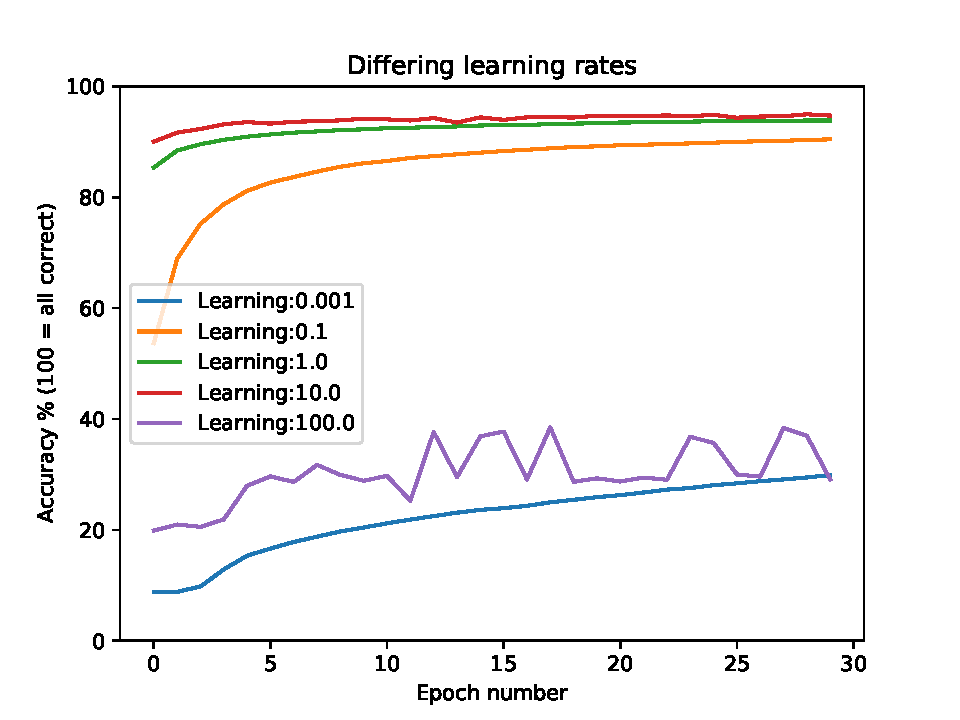
\includegraphics[scale=1]{learningGraph.pdf}
    \caption{
        Varying learning rates for the data. Tested on xTest1 and yTest1. Note
        that the epochs start at 0 not 1
    }
    \label{learning}
\end{figure}

\newpage

The graph of varying batch sizes is in Figure \ref{batchGraph}, as visible the
number of batches has a much less pronounced effect on the accuracy. However, it
is visible that doing batches does have an effect as having a batch size of 1
is visibly much worse than others. In the end, it appears a batch size of 20 was
the best by epoch 30, however, it is very close to the other results.

\begin{figure}[ht]
    \centering
    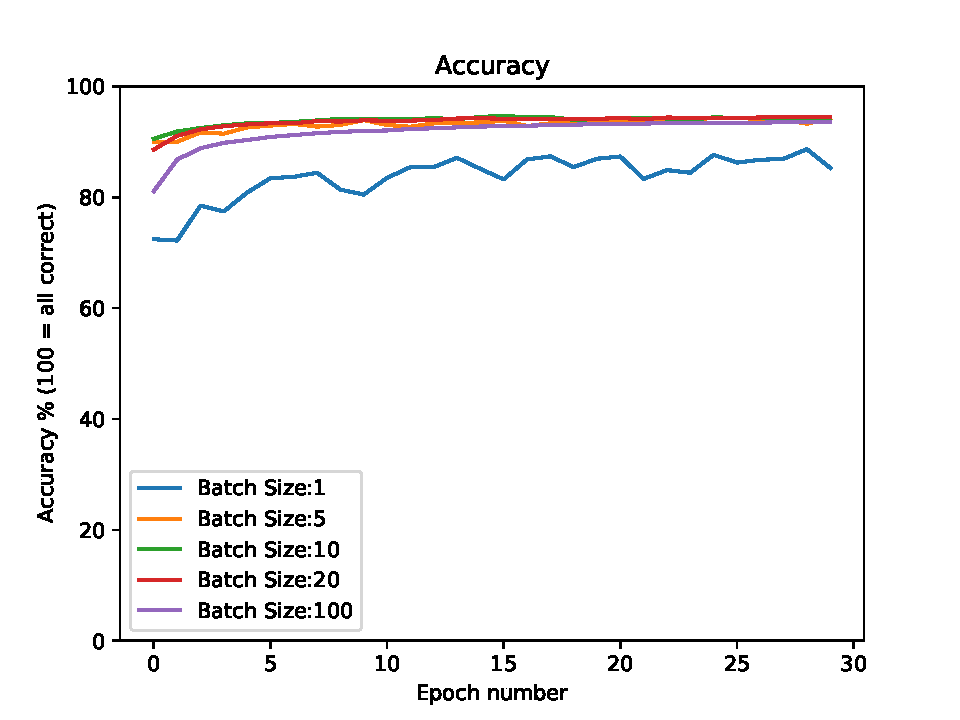
\includegraphics[scale=1]{batchGraph.pdf}
    \caption{
        Varying batch sizes graph for the model. Tested on xTest1 and yTest1.
        Note that the epochs start at 0, not 1
    }
    \label{batchGraph}
\end{figure}

Typically varying batch size has minimal effect and the
learning rate seems to have a golden spot somewhere between 1 and 20. To push
this towards 100\%, the learning rate would probably simply have to be cooled
over time and ran for a much higher number of epochs - essentially simulated
annealling to explore the problem space. \\ \\
\newpage
In Figure \ref{refinedLearning} the idea of this being the golden range is
explored further, and a learning rate of 5 appears to be the best. To further
refine, the learning rates would be set with [1, 2.5, 5, 7.5, 10] as outside of
this there is a visible drop in accuracy in the graph.

\begin{figure}[ht]
    \centering
    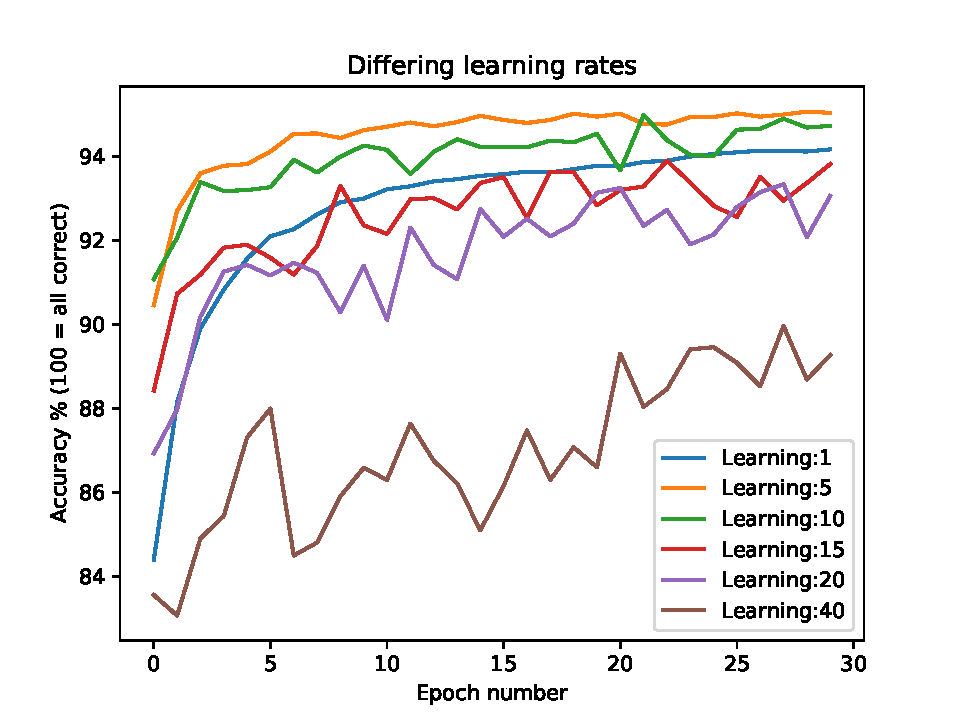
\includegraphics[scale=1]{learningGraphRefined.pdf}
    \caption{
        Varying learning rates graph for the model. Tested on xTest1 and yTest1.
        Note that the epochs start at 0, not 1. This graph contains the highest
        overall accuracy at 94.73\%, but its output was not saved.
    }
    \label{refinedLearning}
\end{figure}

\newpage
Finally, the other approach that was taken was reducing the learning rate
significantly (0.5) and increasing the number of epochs (200) with a batch size
of 15. It only achieved 94.42\%, so it likely got stuck in a bad dip. It's
accuracy over time is visible in Figure \ref{longlong}

\begin{figure}[ht]
    \centering
    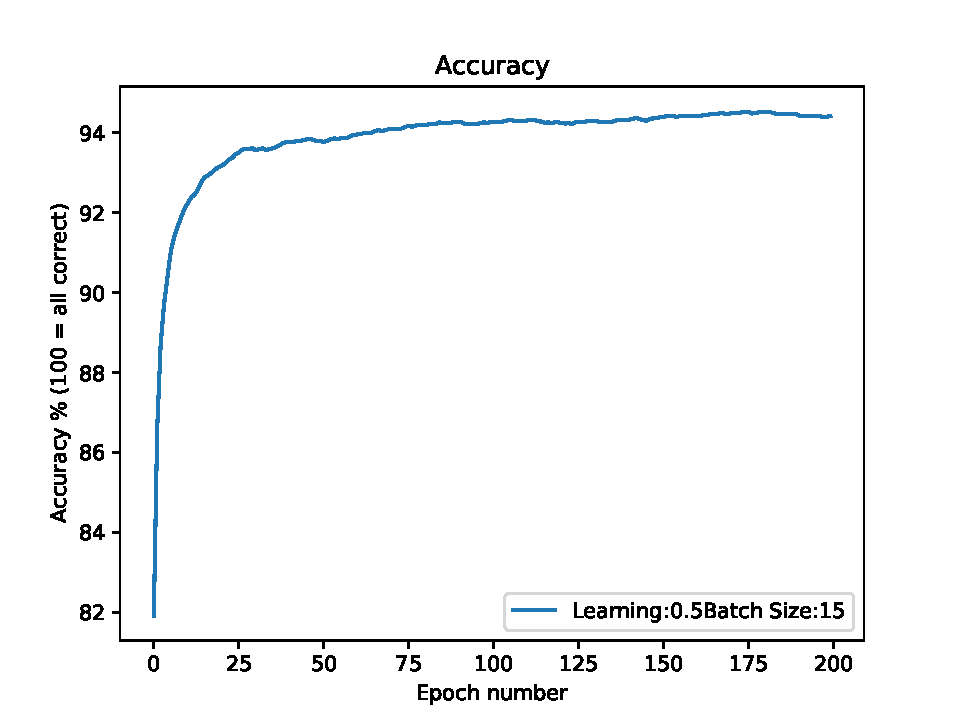
\includegraphics[scale=1]{longlong.pdf}
    \caption{
        Large number of epochs (200) and low learning rate (0.5)
    }
    \label{longlong}
\end{figure}

\newpage
\section{Sign off note}
*this is a leftover comment I wrote while waiting for graphs to generate. It's
informal and is not a part of the actual assessment piece about the quality of the
assessment, and some ideas on how to fix this from a student's experience with 
doing it. Feel free to skip it if you're in a rush to mark, but keep in mind
that its here. 
\\ \\
This assignment was a mess! But it was a fun one after finishing the manual 
calculations by hand. Machine learning is generally finicky, and trying to do
something like this on such a low level (not using PyTorch or Tensorflow) is a
challenge to do properly. After the model was done, it took about 10 hours of
debugging to get it right. Below are some thoughts about changing the teaching
of the maths section or the assessed maths section, the resources provided to
students, and the approach to teaching the topic. Yes, we are in hard times, 
but there are issues with this assessment piece that I hope the staff 
fix before the next time this course is ran. \\ \\
A change to recommend to this in the future is to either show us how to do the
manual calculations with matrix maths (this would help a lot of people with the
coding part), or reduce the manual calculation to only finding a single updated
weight (did you have fun checking my maths?). \\ \\
Additionally, the resources on how to do this... just did not work. The example
pdf skipped the working for several weights and never updated the biases. 
The lab's explanation, while pretty good for how it works, simply does not work 
to follow to actually calculate this many weights. Majority of people in this 
course do not know what a partial derivative is, and spitting a mess of of 
Greek symbols is not simple enough. \\ \\
Overall, this assignment should probably be way more practical. Even if someone
followed the provided materials to point (I actually made a model like this then
abandoned it) it would take 30mins+ to train a single model when we need to
train 10+ models for the basic set of graphs in part 2. \\

A small note is that this assignment is bottlenecked by the computing power
available to students. This is partially a reason why I wanted to actually use
C++ here (we aren't even using any specific python packages?) as with C++ I can
use the -O3 optimisation level or -oFast and the processing time drops by a
factor of ten. My training time was about 5 seconds per epoch, or 2mins 30secs 
per NN with 30 epochs on a Ryzen 3600 (6c12t at 4.2GHz boosted), and that's
quite a high end CPU for people. Provide remote computing on campus, offer
alternatives, make the NN smaller, use C++, make the dataset smaller, etc. \\ \\
If I were to fully redefine this course, I'd change it to be fully (or partly)
hosted on Google Colaboratory - cloud computing, report has the code mixed in,
and the maths can be in a separate document. While its a useful skill to write
LaTeX formulas like this (this document is at 1200 lines! with 1000 being
maths!), writing a smaller number of them (or doing it by hand) would have a
 massive effect on how enjoyable the assignment is. 
    \\ \\
All in all, the assignment took somewhere between 35-40 hours. Including
starting this document in word, realising it won't be fast enough, writing the
code as directed in the assignment, and realising it won't be fast enough as
well. Then swapping over to this (about 15hrs maths, 25 hours coding). 
\\ \\ \\ \\

Good luck and have fun marking the rest of these papers!

\end{document}